\chapter{Flutter}
\section{Flutter Install}
\subsection{System Requirements in Linux}
To install and run Flutter, your development environment must meet these minimum requirements:\\
\begin{itemize}
	\item Operating Systems: Linux (64-bit)
	\item Disk Space: 600 MB (does not include disk space for IDE/tools).
	\item Tools: Flutter depends on these command-line tools being available in your environment.
	\item Shared libraries: Flutter test command depends on this library being available in your environment.
\end{itemize}

\subsection{Get the Flutter SDK}
The easiest way to install Flutter on Linux is by using snapd. For more information, see Installing snapd.\\
Once you have snapd, you can install Flutter using the Snap Store, or at the command line:
\begin{lstlisting}[language=C]
	 sudo snap install flutter --classic
\end{lstlisting}
\textbf{Note: }Once the snap is installed, you can use the following command to display your Flutter SDK path:
\begin{lstlisting}[language=C]
	 flutter sdk-path
\end{lstlisting}

\subsection{Run flutter doctor}
Run the following command to see if there are any dependencies you need to install to complete the setup (for verbose output, add the -v flag):
\begin{lstlisting}[language=C]
	 flutter doctor
\end{lstlisting}
This command checks your environment and displays a report to the terminal window. The Dart SDK is bundled with Flutter; it is not necessary to install Dart separately. 
\subsection{Update your path}
You can update your PATH variable for the current session at the command line, as shown in Get the Flutter SDK.
You'll probably want to update this variable permanently, so you can run flutter commands in any terminal session.

\section{Android setup}
\begin{itemize}
	\item \textbf{Install Android Studio}\\
	1. Download and install Android Studio.\\
	2. Start Android Studio, and go through the 'Android Studio Setup Wizard'. This installs the latest Android SDK, Android SDK Command-line Tools, and Android SDK Build-Tools, which are required by Flutter when developing for Android.\\
	3. Run flutter doctor to confirm that Flutter has located your installation of Android Studio. If Flutter cannot locate it, run flutter config --android-studio-dir <directory> to set the directory that Android Studio is installed to.\\
	\item \textbf{Set up your Android device}\\
	To prepare to run and test your Flutter app on an Android device, you need an Android device running Android 4.1 (API level 16) or higher.\\
	Enable Developer options and USB debugging on your device. Detailed instructions are available in the Android documentation.\\
	\item \textbf{ Agree to Android Licenses}\\
	Before you can use Flutter, you must agree to the licenses of the Android SDK platform. This step should be done after you have installed the tools listed above.
	1.Make sure that you have a version of Java 8 installed and that your 
	\begin{lstlisting}
	JAVA_HOME \end{lstlisting}
	 environment variable is set to the JDK’s folder.\\
	Android Studio versions 2.2 and higher come with a JDK, so this should already be done.  \\
	2. Open an elevated console window and run the following command to begin signing licenses.
	\begin{lstlisting}[language=C]
		flutter doctor --android-licenses\end{lstlisting}
	3. Review the terms of each license carefully before agreeing to them.\\
	4. Once you are done agreeing with licenses, run flutter doctor again to confirm that you are ready to use Flutter.\\	
\end{itemize}
\section{Create the app}
1. Open the IDE and select Create New Flutter Project.\\
2. Select Flutter Application as the project type. Then click Next.\\
3. Verify the Flutter SDK path specifies the SDK’s location (select Install SDK… if the text field is blank).\\
4. Enter a project name (for example, myapp). Then click Next.
Click Finish.
5. Wait for Android Studio to install the SDK and create the project.

\section{Write your first Flutter app}
Firstly, Create a simple, templated Flutter app.\\
We’ll mostly edit lib/main.dart, where the Dart code lives.\\
Replace the contents of lib/main.dart according to the need.\\
Run the app in the way your IDE describes. You should see either Android, iOS, or web output, depending on your device.\\
\lstinputlisting[language=C,style=mystyle, label=dart/makemytripdart]{dart/Session8.dart}
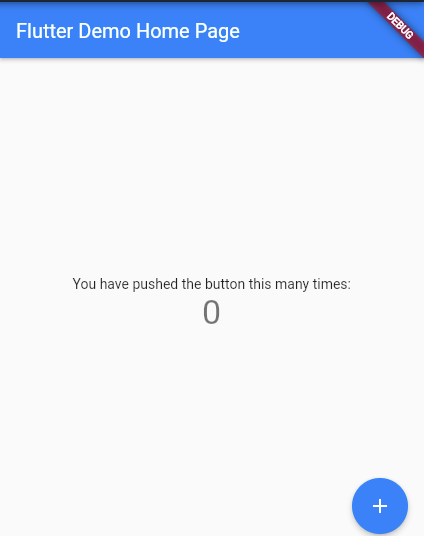
\includegraphics[width=16cm]{dart/flutterdemo.png}\\[0.5cm]
\subsection{Loader}
\lstinputlisting[language=C,style=mystyle, label=dart/Assignment2Loader]{dart/Assignment2Loader}
\begin{center}

\includegraphics[width=8cm, height=8cm]{dart/loader.png}\\[0.5cm]
\end{center}


